\documentclass{article}
\usepackage[utf8]{inputenc}
\usepackage[T1]{fontenc}
\usepackage[spanish]{babel}
\usepackage{hyperref}
\usepackage{float}
\usepackage{url}
\usepackage{booktabs}
\usepackage{amsfonts}
\usepackage{amsmath}
\usepackage{nicefrac}
\usepackage{microtype}
\usepackage{graphicx}
\usepackage{caption}
\usepackage{listings}
\usepackage{color}
\graphicspath{{./images/}}
\usepackage{lmodern}  % Latin Modern, versión escalable de Computer Modern
\usepackage[margin=2.5cm]{geometry}

\title{Trabajo Práctico 1.2 -- Simulación}
\author{
    Renzo Aimaretti \\ \texttt{renzoceronueve@gmail.com}
    \and
    Facundo Sosa Bianciotto \\ \texttt{facundososabianciotto@gmail.com}
    \and
    Vittorio Maragliano \\ \texttt{maraglianovittorio@gmail.com}
    \and
    Ignacio Amelio Ortiz \\ \texttt{nameliortiz@gmail.com}
    \and
    Nicolás Roberto Escobar \\ \texttt{escobar.nicolas.isifrro@gmail.com}
    \and
    Juan Manuel De Elia \\ \texttt{juanmadeelia@gmail.com}
}

\begin{document}
\maketitle

\begin{abstract}
Este trabajo tiene como objetivo el análisis económico-matemático de estrategias de apuestas en la ruleta, abordado desde la perspectiva del apostador mediante simulaciones computacionales. Se desarrolla un simulador en Python 3.x que reproduce el comportamiento del juego y permite implementar diversas estrategias clásicas como Martingala, D’Alembert , Fibonacci y Paroli. El estudio contempla dos escenarios contrastantes: capital acotado (realista) y capital infinito (idealizado), con especial atención a la frecuencia de bancarrota en el primero. Los resultados obtenidos son representados gráficamente utilizando herramientas como Matplotlib, permitiendo evaluar la efectividad y el riesgo de cada estrategia a través de múltiples ejecuciones. Este enfoque busca desmitificar la posibilidad de obtener beneficios sistemáticos en la ruleta.
\end{abstract}

\section{Introducción}
Utilizamos Python para crear una ruleta simulada y probamos varias formas de apostar, entre ellas tres estrategias conocidas: Martingala, D’Alembert y Fibonacci. Además, agregamos una cuarta estrategia que se usa bastante en la práctica pero que no siempre se estudia tanto desde un punto de vista matemático: la estrategia Paroli, también conocida como la "anti-martingala", donde en vez de doblar la apuesta al perder, se la dobla cuando se gana, y en la cual se recomienda luego de 3 o 4 jugadas ganadas volver a la apuesta inicial.

Nuestro objetivo no es solo ver si se gana o se pierde, sino entender cómo se comportan estas estrategias cuando se juega con capital limitado (como en la vida real) y cuando se supone un capital infinito (más ideal). También analizamos cuántas veces el jugador termina en bancarrota y qué tan rápido pasa eso dependiendo de la estrategia. A lo largo del trabajo mostramos los resultados mediante gráficos, sacamos conclusiones y reflexionamos sobre si realmente existe una forma "inteligente" de apostar, o si al final la ruleta sigue siendo un juego de azar, por más cálculos que hagamos.

En este informe, vamos a simular la ruleta con una apuesta de \$10, y teniendo en cuenta que el apostador puede realizar los distintos tipos de apuesta:
\begin{itemize}
    \item Apostar a un número específico (0-36).
    \item Apostar a un color(rojo o negro)
    \item Apostar a una docena(primer docena, segunda docena,tercer docena)
    \item Apostar a una fila(primera fila,segunda fila o tercera fila del tablero)
    \item Apostar a numero par o numero impar
    \item Apostar a numero alto o numero bajo(del 1 al 18 o del 19 al 36)
\end{itemize}
La apuesta que se decida realizar va a ingresarse por argumento en la consola
\subsection{Justificación del número de corridas: Teorema Central del Límite}

En este trabajo se realizaron 30 corridas independientes para cada combinación de estrategia y condición de capital (finito e infinito). Esta elección se fundamenta teóricamente en el \textbf{Teorema Central del Límite (TCL)}, uno de los pilares fundamentales de la estadística inferencial.

El Teorema Central del Límite establece que, dado un número suficientemente grande de muestras independientes y aleatorias de una población con una media $\mu$ y desviación estándar $\sigma$ finitas, la distribución de la media muestral tenderá a una distribución normal, independientemente de la forma de la distribución original de la población.

En particular, el TCL permite aproximar la distribución de cualquier estadístico (como el capital final o la tasa de éxito promedio) mediante una distribución normal cuando se cuenta con un tamaño de muestra significtiva. Aunque no existe un umbral fijo, en la práctica estadística se considera que un número de muestras igual o superior a 30 suele ser suficiente para que esta aproximación sea válida, incluso cuando la distribución original es asimétrica o discreta.

\noindent
\textbf{Ventajas de usar 30 corridas:}
\begin{itemize}
    \item Permite calcular medias y desviaciones estándar muestrales con una estimación robusta.
    \item Facilita el uso de herramientas estadísticas como intervalos de confianza o pruebas de hipótesis.
    \item Reduce la variabilidad atribuida a una única simulación, mejorando la representatividad de los resultados.
\end{itemize}

\noindent
\textbf{Aplicación en este estudio:} Cada corrida representa una simulación independiente de una estrategia de apuestas bajo condiciones aleatorias. Al realizar 30 de estas corridas, obtenemos una muestra suficientemente grande para estudiar el comportamiento promedio de cada estrategia y analizar su variabilidad. Esto nos permite comparar estrategias de forma más confiable y realizar generalizaciones sobre su desempeño típico.

\begin{center}
    \textit{En conclusion, se utilizan 30 corridas para garantizar una base estadística sólida, aprovechar la validez del Teorema Central del Límite y permitir inferencias representativas sobre el comportamiento de cada estrategia.}
\end{center}
    
\section{Descripción del programa}
\subsection{Funciones del programa}
El programa está compuesto por varias funciones, destacandose la funcion jugar, la cual dependiendo de la jugada que se decida realizar va a llamar a las distintas funciones para cada juego. A continuación, se describe cada una de ellas en detalle.

\subsection{Conceptos teóricos utilizados}
Se emplearon las siguientes formulas de estadistica:
1. Frecuencia relativa real:
\[
f_{\text{real}} = \frac{n_{\text{real}}}{n_{\text{total}}}
\]
donde \( n_{\text{real}} \) es la frecuencia observada y \( n_{\text{total}} \) es el total de observaciones.

Se utilizaron las siguientes estrategias de apuestas, apostando a numeros pares:
1.Fibonacci : 
Se utiliza la secuencia de Fibonacci para determinar el monto de la apuesta. La secuencia comienza con 1 y 1, y cada número siguiente es la suma de los dos anteriores. Si se pierde, se avanza un número en la secuencia; si se gana, se retrocede dos números en la secuencia.
Se emplea tambien el concepto teorico de la secuencia de Fibonacci, la cual es : 1,1,2,3,5,8,13,21,34,55,89,144....
2.Martingala :
Para la estrategia Martingala se duplica la apuesta después de cada pérdida, y se vuelve a la apuesta inicial después de una victoria. Esta estrategia busca recuperar las pérdidas anteriores con una sola victoria.
3.D’Alembert:
La estrategia D'Alembert aumenta la apuesta en una unidad después de una pérdida y la disminuye en una unidad después de una victoria. Esta estrategia busca equilibrar las ganancias y pérdidas a lo largo del tiempo.
4.Paroli : 
La estrategia Paroli duplica la apuesta luego de cada victoria y vuelve a la apuesta inicial después de una pérdida. Esta estrategia busca maximizar las ganancias durante una racha ganadora.

\subsubsection{simular\_ruleta}
La función \texttt{simular\_ruleta} es la encargada de generar la tirada de la ruleta, simulando el lanzamiento de la bola y obteniendo un número aleatorio entre 0 y 36. Esta función utiliza la biblioteca \texttt{random} de Python para generar números aleatorios:

\begin{verbatim}
def simular_ruleta():
    return random.randint(0, 36)
\end{verbatim}

\subsubsection{estrategia}
Esta función determina el monto de la próxima apuesta basándose en diferentes algoritmos según la estrategia seleccionada:

\begin{verbatim}
def estrategia(apuesta_actual, historial, gano, tipo):
    if tipo == 'm':
        return apostar_martingala(apuesta_actual, gano), historial
    elif tipo == 'd':
        return apostar_dalembert(apuesta_actual, gano), historial
    elif tipo == 'f':
        nueva_apuesta, nuevo_historial = apostar_fibonacci(historial, gano)
        return nueva_apuesta, nuevo_historial
    elif tipo == 'p':
        return apostar_paroli(apuesta_actual, gano), historial
    else:
        raise ValueError("Estrategia no reconocida")
\end{verbatim}

Recibe como parámetros:
\begin{itemize}
    \item \texttt{apuesta\_actual}: Monto de la apuesta actual.
    \item \texttt{historial}: Lista con el historial de apuestas anteriores.
    \item \texttt{gano}: Booleano que indica si se ganó (True) o perdió (False) la última apuesta.
    \item \texttt{tipo}: Tipo de estrategia a aplicar ('m' para Martingala, 'd' para D'Alembert, 'f' para Fibonacci o 'p' para Paroli).
\end{itemize}

Retorna una tupla con dos elementos:
\begin{itemize}
    \item El monto de la próxima apuesta calculado según la estrategia elegida.
    \item El historial de apuestas actualizado (relevante para la estrategia Fibonacci).
\end{itemize}

\subsection{jugar}
La función \texttt{jugar} tiene como propósito simular una sesión de apuestas en la ruleta, siguiendo una estrategia determinada, durante un número fijo de tiradas. Su diseño permite evaluar el comportamiento del capital a lo largo del tiempo y calcular la frecuencia relativa de aciertos en función de los resultados obtenidos.

\begin{verbatim}
    def jugar(tiradas, numero_elegido, tipo_estrategia, capital_tipo, capital_inicial)
\end{verbatim}

\noindent Los parámetros de entrada son:
\begin{itemize}
    \item \texttt{tiradas}: cantidad total de jugadas a simular.
    \item \texttt{numero\_elegido}: apuesta seleccionada (puede ser un número específico, una docena, una fila, par/impar, rojo/negro, número bajo/alto).
    \item \texttt{tipo\_estrategia}: estrategia de progresión aplicada (puede ser Martingala, Fibonacci, D’Alembert o Paroli).
    \item \texttt{capital\_tipo}: especifica si el capital es \texttt{fijo} o \texttt{infinito}. Si es \texttt{infinito}, el capital se reinicia cada vez que se agota.
    \item \texttt{capital\_inicial}: cantidad de dinero inicial disponible para apostar.
\end{itemize}

Durante la simulación, se ejecutan las siguientes acciones principales:
\begin{enumerate}
    \item Se inicializa el capital y la apuesta base.
    \item Por cada tirada, se simula un resultado de ruleta y se evalúa si se ha ganado la apuesta según la apuesta elegida.
    \item En caso de acierto, se incrementa el capital según el tipo de apuesta (pago 1:1, 2:1 o 35:1). En caso contrario, se descuenta el monto apostado.
    \item La progresión de la apuesta se ajusta conforme a la estrategia elegida.
    \item En caso de que el capital disponible no sea suficiente para realizar la siguiente apuesta y el tipo de capital no sea infinito, se considera que el jugador ha entrado en \textit{banca rota}, lo que implica la finalización inmediata de la simulación de la corrida actual. Para mantener la coherencia estructural con otras corridas que sí completaron la totalidad de las tiradas, el historial de capital se completa artificialmente con el último valor de capital (que en este caso es cero) hasta alcanzar la longitud total de tiradas especificada. Esto permite un análisis gráfico homogéneo y evita desfases en las comparaciones visuales entre corridas.
    \item Se almacena el capital luego de cada tirada.
\end{enumerate}

Al finalizar, se construye un historial de capital y se calcula la \textbf{frecuencia relativa de éxito acumulada} (\texttt{frsa}), que indica la proporción de tiradas en las que el resultado fue favorable respecto a la cantidad de tiradas hasta el momento.

\noindent La función retorna:
\begin{itemize}
    \item \texttt{capital\_historial}: evolución del capital a lo largo de las tiradas.
    \item \texttt{banca\_rota}: valor booleano que indica si el capital se agotó.
    \item \texttt{frsa}: arreglo con la frecuencia relativa acumulada de aciertos por tirada.
\end{itemize}

\subsection*{Visualización de resultados: funciones de graficación}
Para facilitar el análisis visual del comportamiento del capital y la frecuencia relativa de éxito a lo largo de las tiradas, se han desarrollado tres funciones específicas de graficación. A continuación, se detalla su propósito y funcionamiento general:

\begin{itemize}
    \item \texttt{graficar\_capital}: Grafica la evolución del capital a lo largo de las tiradas.
    \item \texttt{graficar\_frsa}: Grafica la frecuencia relativa de aparición de la opcion elegida.
    \item \texttt{graficar\_todas\_corridas}: Grafica la evolución del capital para todas
\end{itemize}

\begin{verbatim}
    def graficar_capital(capital_historial, titulo, nombre_archivo):
    plt.figure(figsize=(10, 6))
    plt.plot(range(1, len(capital_historial)+1), capital_historial, color='red')
    plt.axhline(y=capital_historial[0], color='blue', linestyle='--', label='Capital Inicial')
    plt.title(titulo)
    plt.xlabel("Tiradas")
    plt.ylabel("Capital")
    plt.grid(True)
    plt.legend()
    plt.savefig(nombre_archivo)
    plt.close()
    
def graficar_frsa(frsa, titulo, nombre_archivo):
    plt.figure(figsize=(8, 5))
    plt.bar(range(1, len(frsa) + 1), frsa, color='salmon', edgecolor='blue')
    plt.title(titulo)
    plt.xlabel("n (número de tiradas)")
    plt.ylabel("frsa (frecuencia relativa)")
    plt.ylim(0, 1)
    plt.grid(True, linestyle='--', alpha=0.5)
    plt.savefig(nombre_archivo)
    plt.close()

def graficar_todas_corridas(historiales_capital, titulo, nombre_archivo):
    plt.figure(figsize=(10, 6))
    for i, capital_historial in enumerate(historiales_capital):
        plt.plot(range(1, len(capital_historial) + 1), capital_historial,
         label=f"Corrida {i + 1}", alpha=0.7)
    plt.axhline(y=historiales_capital[0][0], color='blue', linestyle='--',
     label='Capital Inicial')
    plt.title(titulo)
    plt.xlabel("Tiradas")
    plt.ylabel("Capital")
    plt.grid(True)
    plt.legend()
    plt.savefig(nombre_archivo)
    plt.close()  
\end{verbatim}

\subsection{Calcular resultado de la tirada}
Estas funciones se ocupan de determiar si el numero que salio en la tirada corresponde una fila, una docena, par, impar, rojo o negro. Se llama una funcion u otra dependiendo el tipo de apuesta realizada por el jugador.

\begin{verbatim}
def get_row(number):
    if number == 0:
        return None
    if number % 3 == 1:
        return "primera"
    elif number % 3 == 2:
        return "segunda"
    else:
        return "tercera"

def get_dozen(number):
    if 1 <= number <= 12:
        return "primera docena"
    elif 13 <= number <= 24:
        return "segunda docena"
    elif 25 <= number <= 36:
        return "tercera docena"
    else:
        return None

def odd_even(number):
    if number == 0:
        return None
    return "par" if number % 2 == 0 else "impar"

def red_black(number):
    if number == 0:
        return None
    if number in [1, 3, 5, 7, 9, 12, 14, 16, 18, 19, 21, 23, 25, 27, 30, 32, 34, 36]:
        return "rojo"
    else:
        return "negro"
\end{verbatim}

\subsubsection{main}
La función principal coordina la ejecución del programa:

\begin{verbatim}
def main():
    parser = argparse.ArgumentParser()
    parser.add_argument("-c", "--corridas", type=int, default=1, help="Número de corridas")
    parser.add_argument("-n", "--tiradas", type=int, default=1000,
     help="Número de tiradas por corrida")
    parser.add_argument("-e", "--elegido", type=str, default='17', help="Número elegido")
    parser.add_argument("-s", "--estrategia", type=str, required=True, 
    help="Estrategia: m (martingala), d (D'Alembert), f (Fibonacci), p (Paroli)")
    parser.add_argument("-a", "--capital", type=str, required=True, 
    help="Capital: f (finito), i (infinito)")
    parser.add_argument("-i", "--inicial", type=int, default=1000, help="Capital inicial")
    args = parser.parse_args()

    banca_rotas = 0
    historiales_capital = []

    for _ in range(args.corridas):
        capital_historial, banca_rota, frsa = jugar(args.tiradas, args.elegido, 
        args.estrategia, args.capital, args.inicial)
        historiales_capital.append(capital_historial)
        if banca_rota or capital_historial[-1] <= 0:
            banca_rotas += 1

    graficar_capital(capital_historial, f"Corrida 
    {args.corridas} - Evolución del Capital", f"capital_corrida_{args.corridas}.png")
    graficar_frsa(frsa, f"Corrida 
    {args.corridas} - Frecuencia Relativa de Aciertos", f"frsa_corrida_{args.corridas}.png")
        
    
    graficar_todas_corridas(historiales_capital, 
    "Evolución del Capital - Todas las Corridas", "capital_todas_corridas.png")
    print(f"Simulación finalizada.")
    print(f"Resultados de la estrategia '{args.estrategia}' con capital '{args.capital}':")
    print(f"Capital inicial: {args.inicial}")
    print(f"Número elegido: {args.elegido}")
    print(f"Número de tiradas por corrida: {args.tiradas}")
    print(f"Número de corridas: {args.corridas}")
    print(f"Total de bancarrotas: {banca_rotas} de {args.corridas} corridas.")

\end{verbatim}

Esta función:
\begin{itemize}
    \item Recibe argumentos de línea de comandos para configurar la simulación (número de corridas, tiradas, número elegido, estrategia, tipo de capital y capital inicial).
    \item Ejecuta la función \texttt{jugar} para cada corrida, almacenando los resultados en una lista.
    \item Genera gráficos de la evolución del capital y la frecuencia relativa de aciertos utilizando las funciones \texttt{graficar\_capital} y \texttt{graficar\_frsa}.
    \item Imprime en la consola un resumen de los resultados obtenidos, incluyendo el número de bancarrotas y el capital final.
    \item Llama a la función \texttt{graficar\_todas\_corridas} para graficar la evolución del capital
    \item Muestra un resumen de los resultados obtenidos, incluyendo el número de bancarrotas y el capital final.
\end{itemize}

\subsection{Resultados y Conclusiones}

A continuación, se presentan los resultados de las simulaciones realizadas con las distintas estrategias de apuestas: Martingala, D’Alembert, Fibonacci y Paroli. Para cada una se consideraron dos escenarios:

\begin{itemize}
    \item \textbf{Capital finito}: se establece un monto inicial de capital, y se detiene la simulación si se alcanza la bancarrota.
    \item \textbf{Capital infinito}: se asume que el jugador puede continuar apostando indefinidamente sin restricción de fondos.
\end{itemize}

Para cada combinación de estrategia y escenario, se muestran las siguientes tres gráficas:

\begin{itemize}
    \item \textbf{Evolución del capital} en una corrida individual.
    \item \textbf{Frecuencia relativa de aciertos (FRSA)} en esa corrida.
    \item \textbf{Evolución del capital en 30 corridas} independientes.
\end{itemize}


% ====================
% Martingala
% ====================
\subsubsection*{Estrategia Martingala}


\begin{figure}[H]
    \centering
    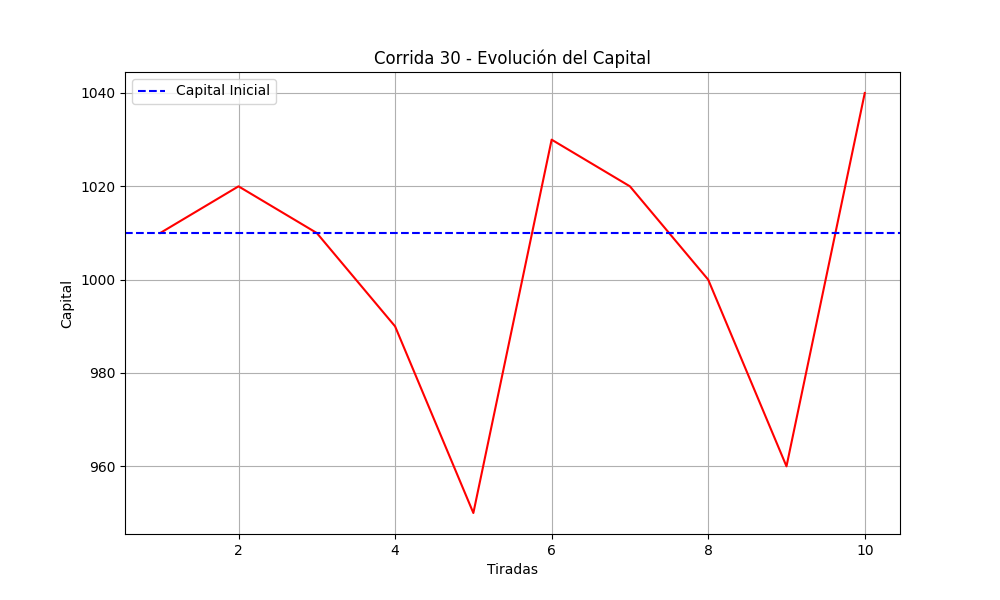
\includegraphics[width=0.8\textwidth]{./images/capital_corrida_30_m_f.png}
    \caption{Martingala (finito) - Evolución del capital en una corrida}
\end{figure}

\begin{figure}[H]
    \centering
    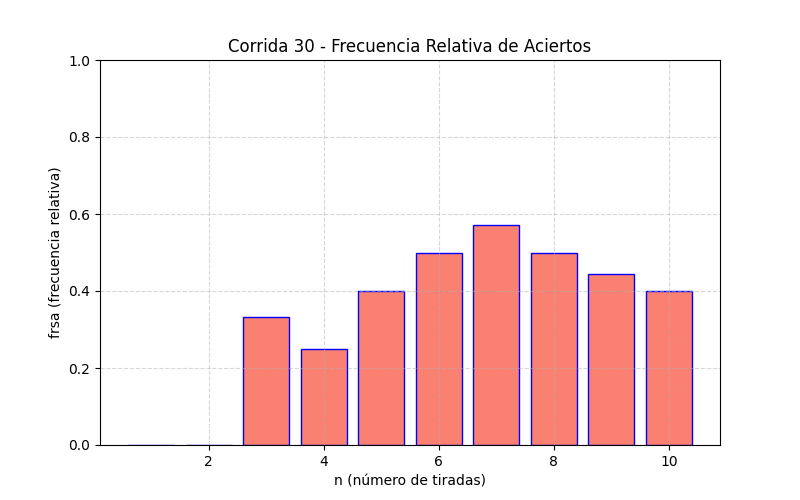
\includegraphics[width=0.7\textwidth]{./images/frsa_corrida_30_m_f.png}
    \caption{Martingala (finito) - Frecuencia relativa de aciertos}
\end{figure}

\begin{figure}[H]
    \centering
    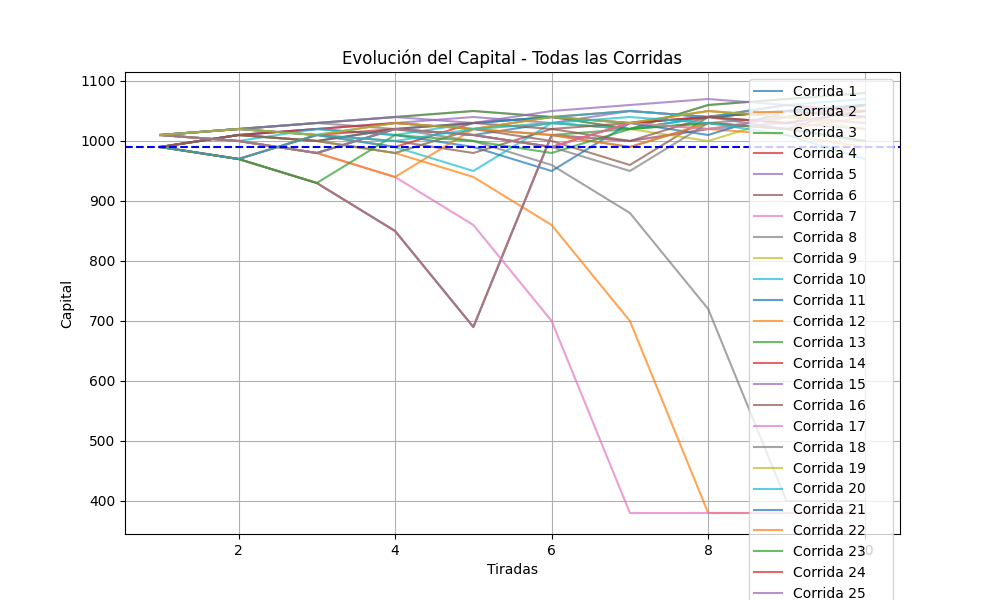
\includegraphics[width=0.85\textwidth]{./images/capital_todas_corridas_m_f.png}
    \caption{Martingala (finito) - Capital en 30 corridas}
\end{figure}


\begin{figure}[H]
    \centering
    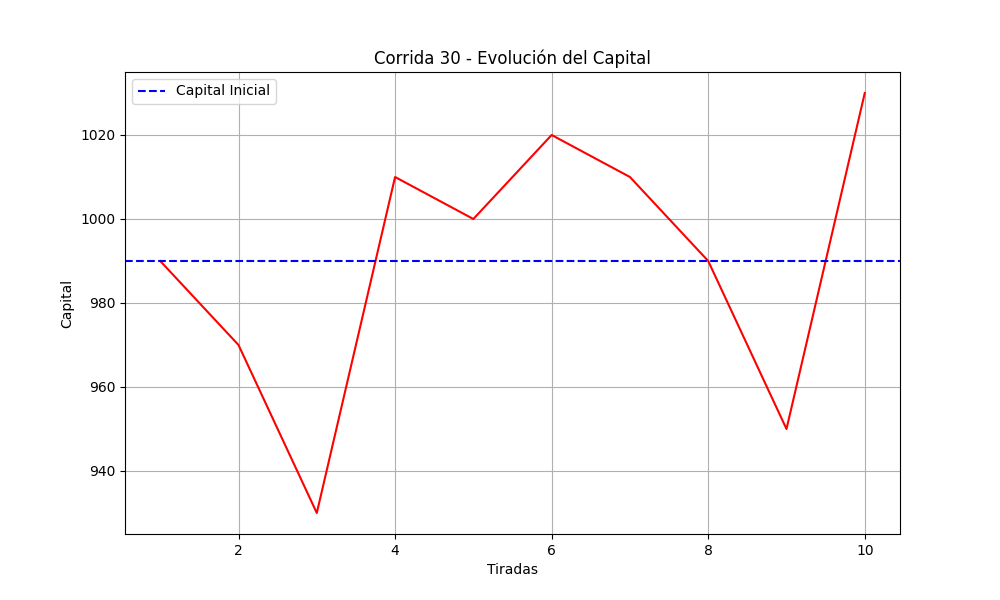
\includegraphics[width=0.8\textwidth]{./images/capital_corrida_30_m_i.png}
    \caption{Martingala (infinito) - Evolución del capital en una corrida}
\end{figure}

\begin{figure}[H]
    \centering
    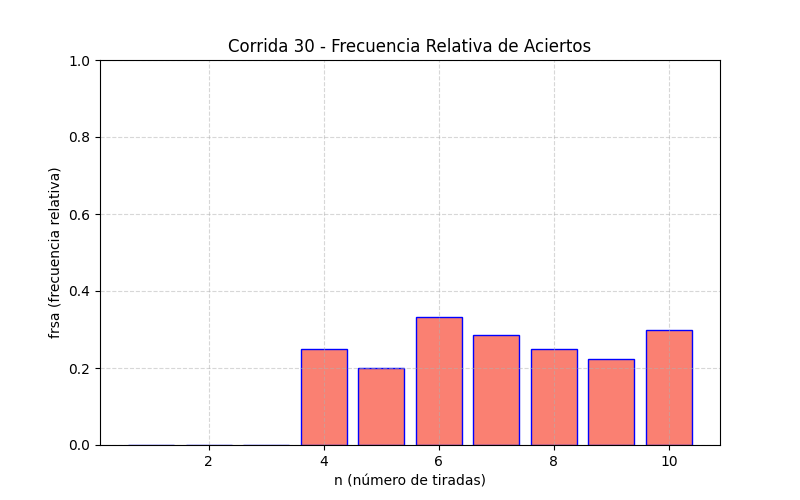
\includegraphics[width=0.7\textwidth]{./images/frsa_corrida_30_m_i.png}
    \caption{Martingala (infinito) - Frecuencia relativa de aciertos}
\end{figure}

\begin{figure}[H]
    \centering
    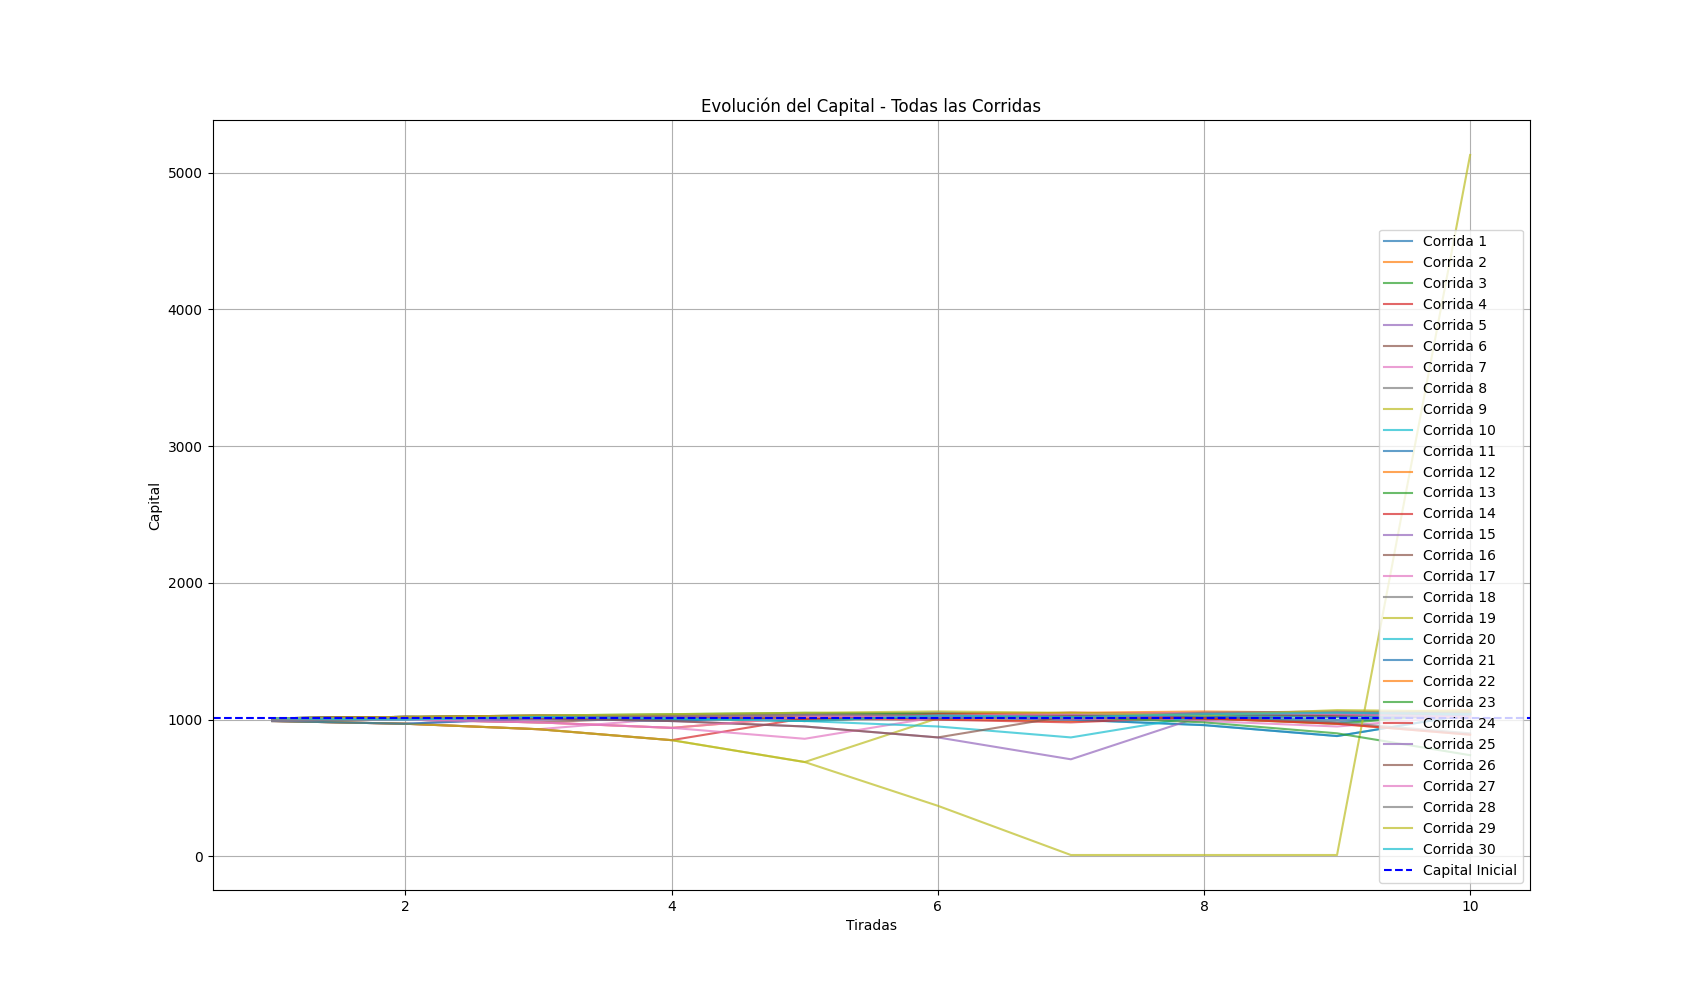
\includegraphics[width=0.85\textwidth]{./images/capital_todas_corridas_m_i.png}
    \caption{Martingala (infinito) - Capital en 30 corridas}
\end{figure}


% ====================
% D'Alembert
% ====================
\subsubsection*{Estrategia D’Alembert}


\begin{figure}[H]
    \centering
    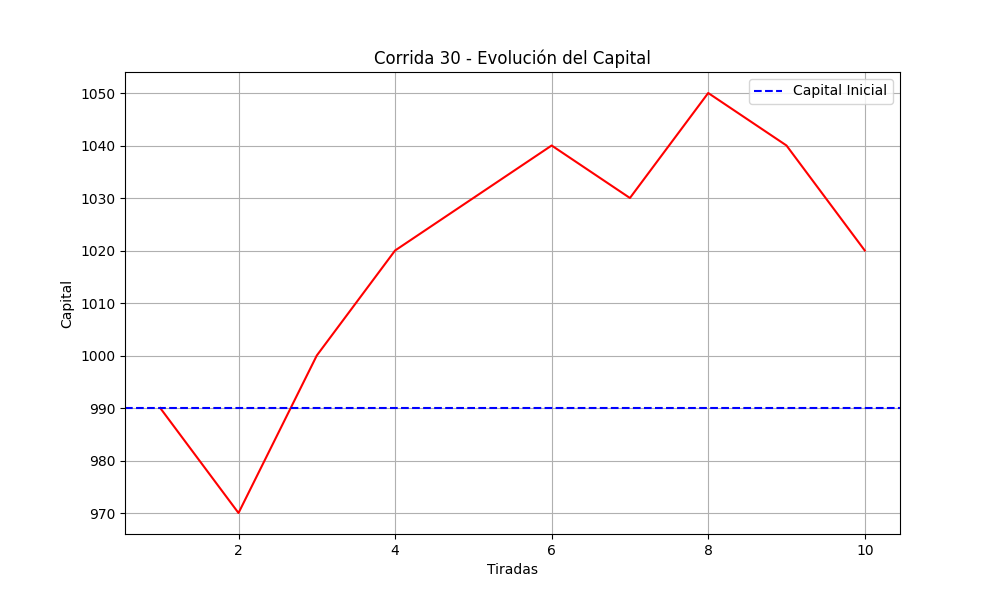
\includegraphics[width=0.8\textwidth]{./images/capital_corrida_30_d_f.png}
    \caption{D’Alembert (finito) - Evolución del capital en una corrida}
\end{figure}

\begin{figure}[H]
    \centering
    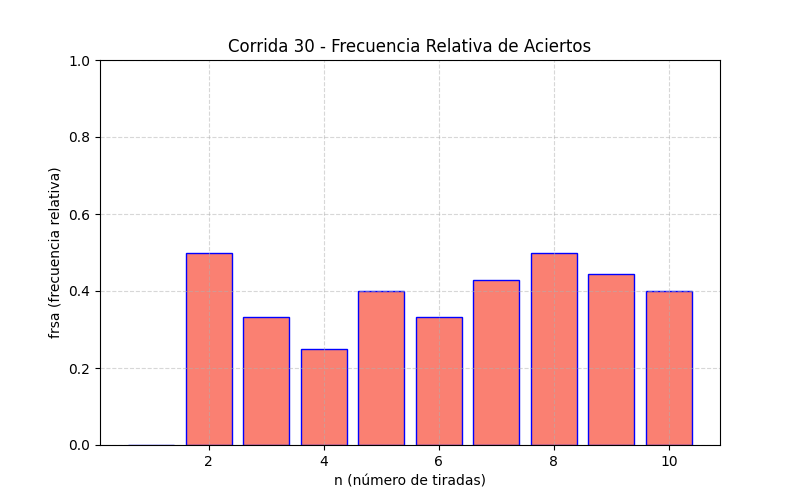
\includegraphics[width=0.7\textwidth]{./images/frsa_corrida_30_d_f.png}
    \caption{D’Alembert (finito) - Frecuencia relativa de aciertos}
\end{figure}

\begin{figure}[H]
    \centering
    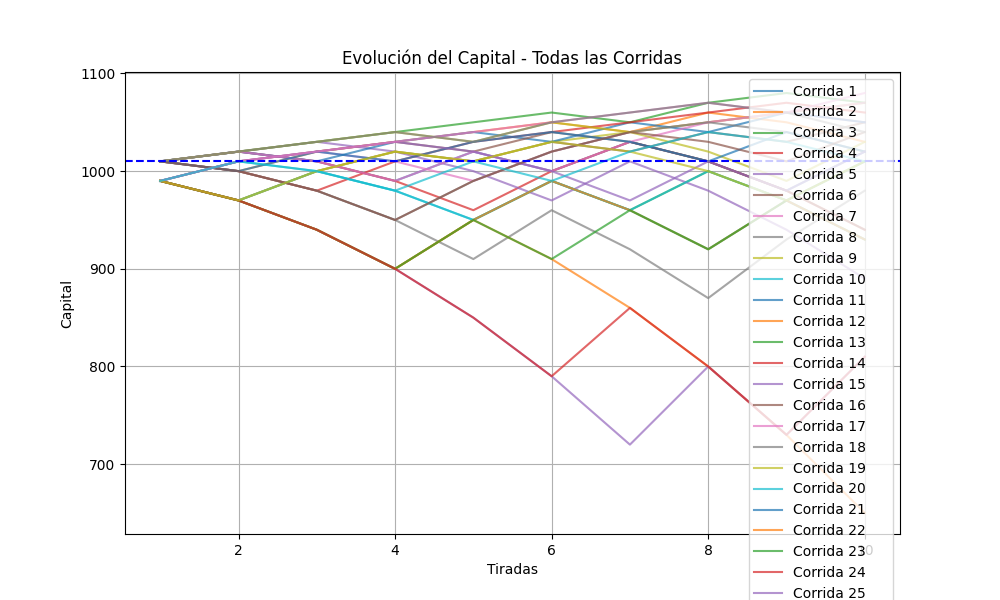
\includegraphics[width=0.85\textwidth]{./images/capital_todas_corridas_d_f.png}
    \caption{D’Alembert (finito) - Capital en 30 corridas}
\end{figure}


\begin{figure}[H]
    \centering
    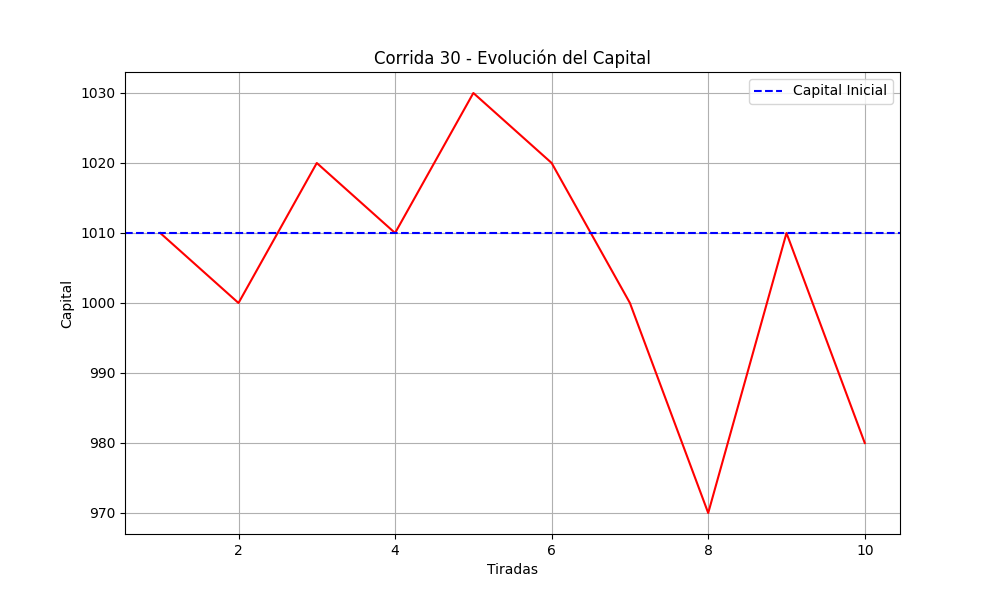
\includegraphics[width=0.8\textwidth]{./images/capital_corrida_30_d_i.png}
    \caption{D’Alembert (infinito) - Evolución del capital en una corrida}
\end{figure}

\begin{figure}[H]
    \centering
    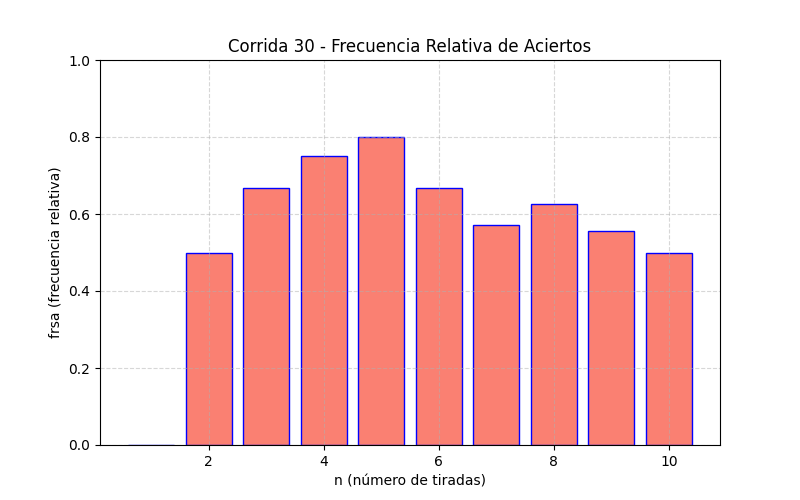
\includegraphics[width=0.7\textwidth]{./images/frsa_corrida_30_d_i.png}
    \caption{D’Alembert (infinito) - Frecuencia relativa de aciertos}
\end{figure}

\begin{figure}[H]
    \centering
    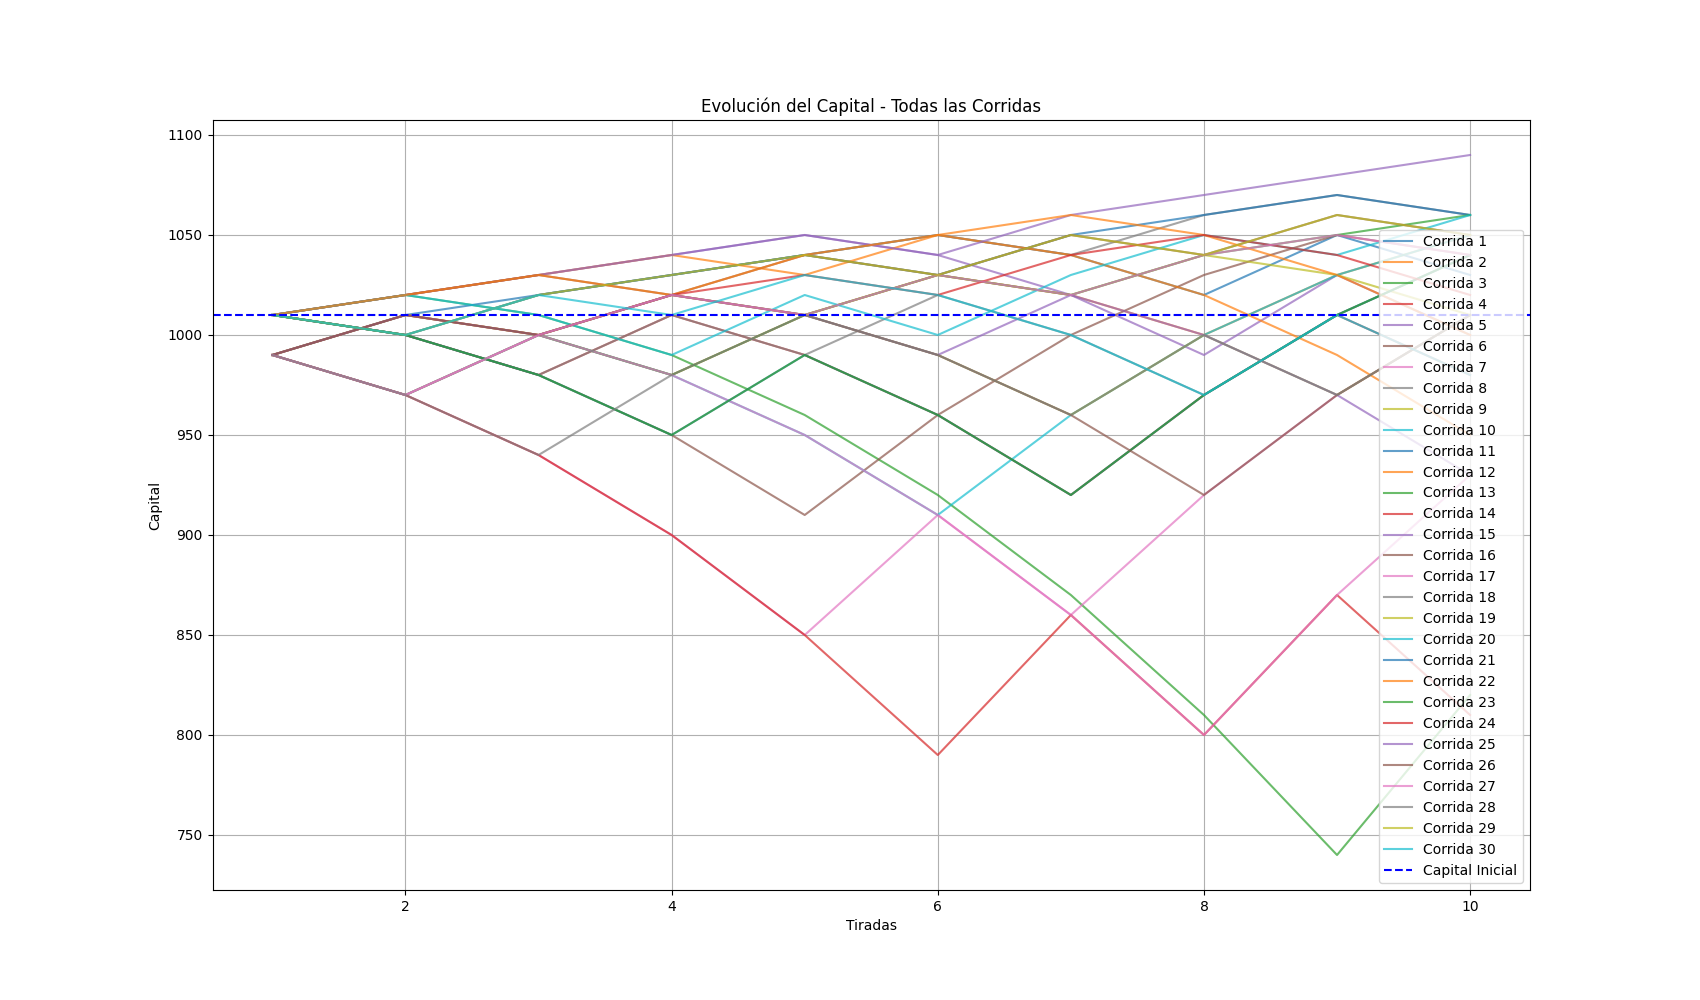
\includegraphics[width=0.85\textwidth]{./images/capital_todas_corridas_d_i.png}
    \caption{D’Alembert (infinito) - Capital en 30 corridas}
\end{figure}


% ====================
% Fibonacci
% ====================
\subsubsection*{Estrategia Fibonacci}


\begin{figure}[H]
    \centering
    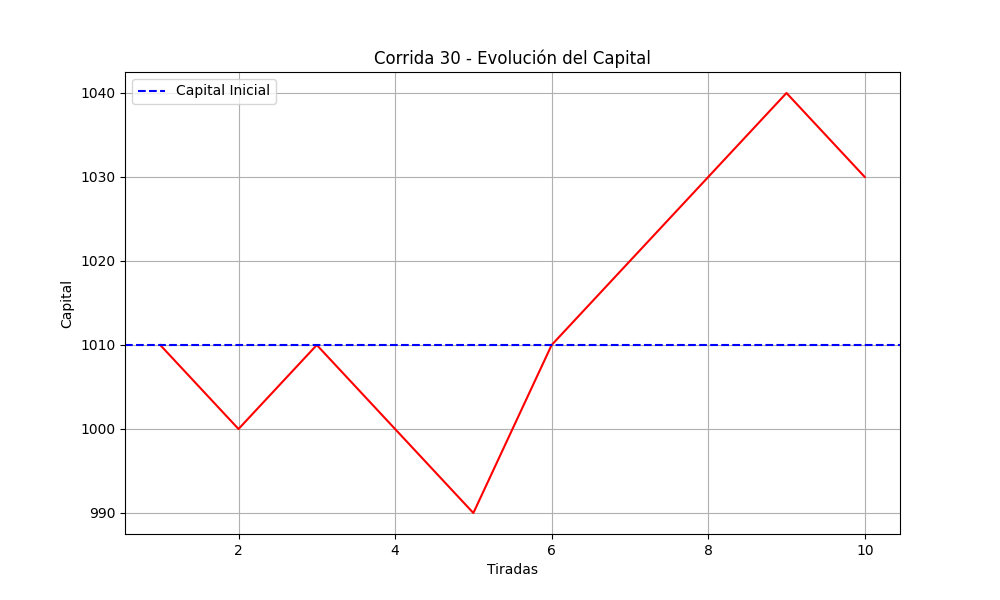
\includegraphics[width=0.8\textwidth]{./images/capital_corrida_30_f_f.png}
    \caption{Fibonacci (finito) - Evolución del capital en una corrida}
\end{figure}

\begin{figure}[H]
    \centering
    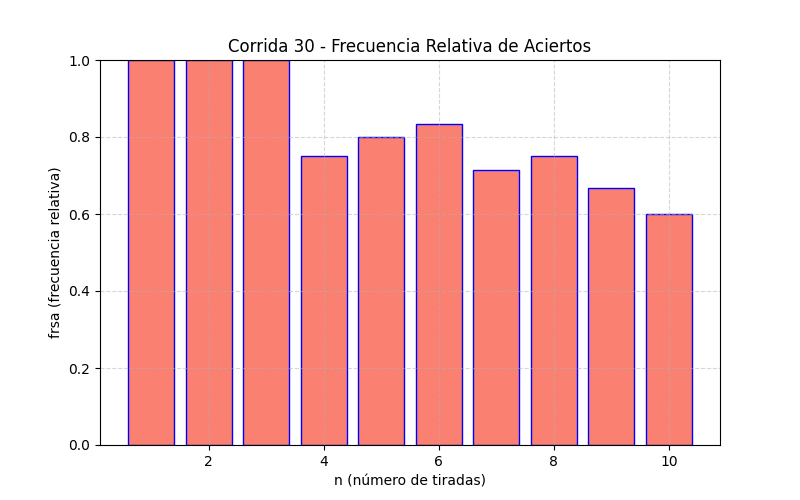
\includegraphics[width=0.7\textwidth]{./images/frsa_corrida_30_f_f.png}
    \caption{Fibonacci (finito) - Frecuencia relativa de aciertos}
\end{figure}

\begin{figure}[H]
    \centering
    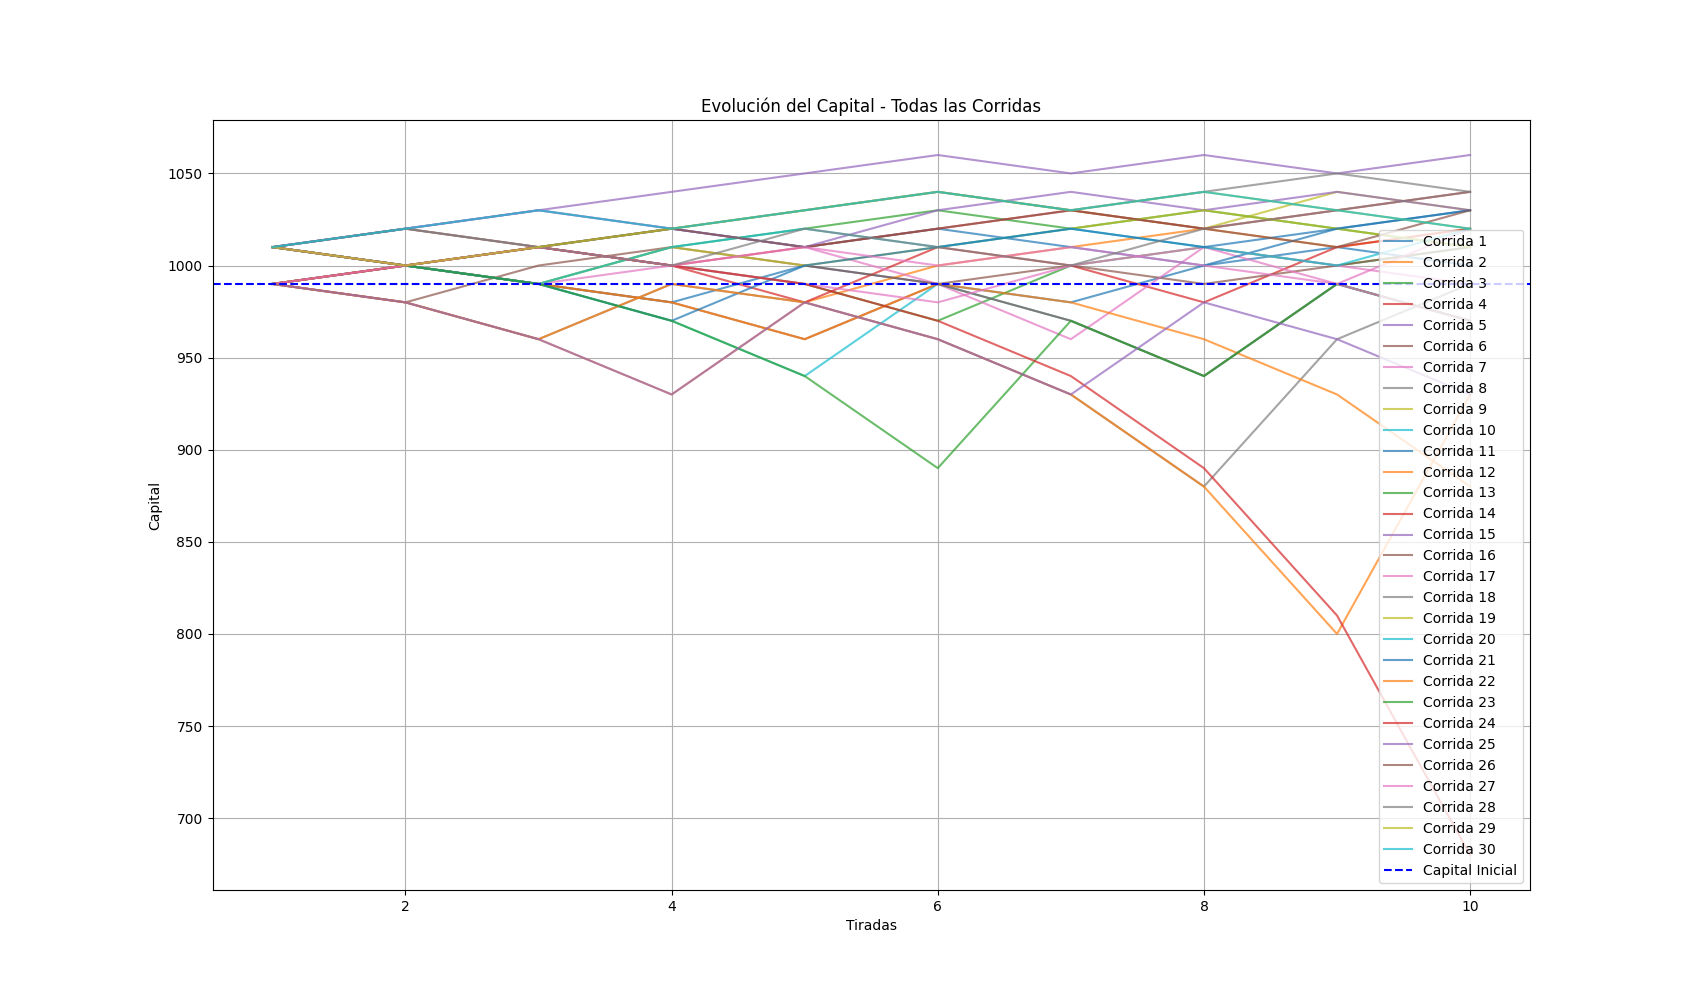
\includegraphics[width=0.85\textwidth]{./images/capital_todas_corridas_f_f.png}
    \caption{Fibonacci (finito) - Capital en 30 corridas}
\end{figure}


\begin{figure}[H]
    \centering
    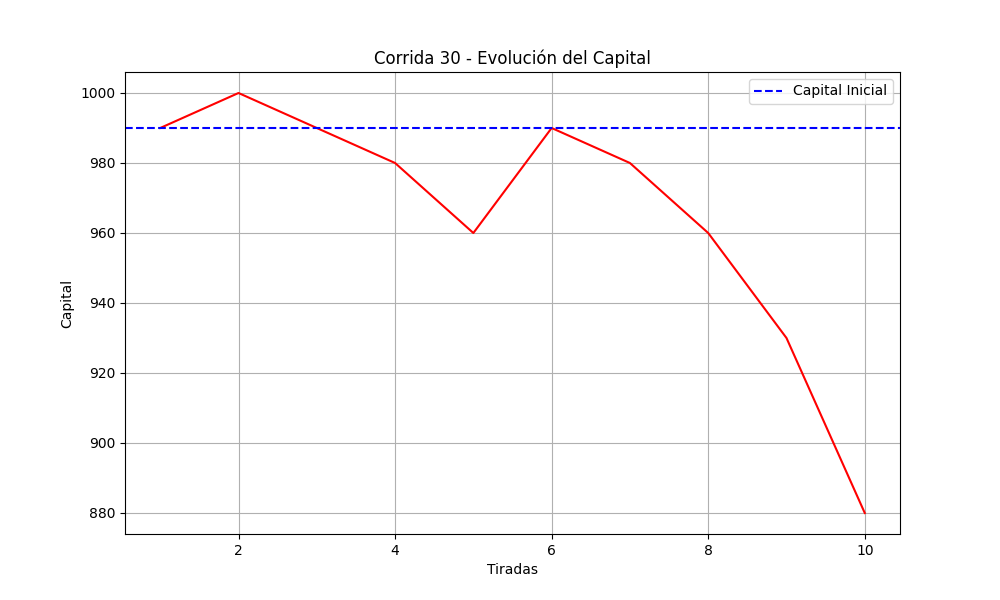
\includegraphics[width=0.8\textwidth]{./images/capital_corrida_30_f_i.png}
    \caption{Fibonacci (infinito) - Evolución del capital en una corrida}
\end{figure}

\begin{figure}[H]
    \centering
    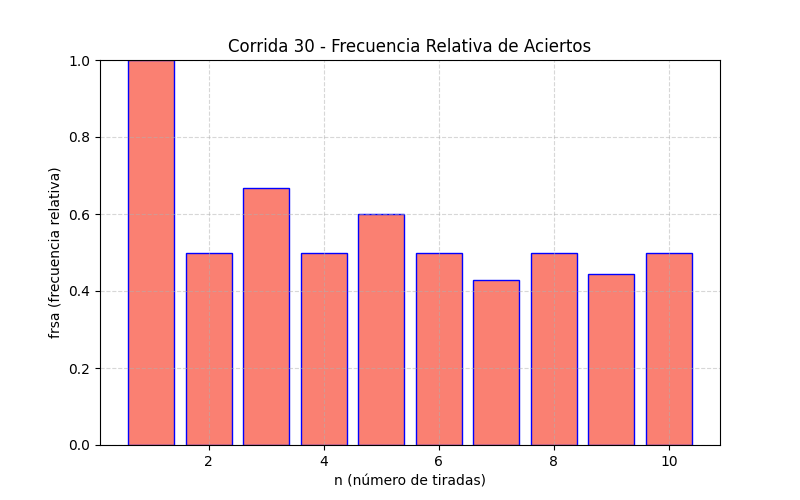
\includegraphics[width=0.7\textwidth]{./images/frsa_corrida_30_f_i.png}
    \caption{Fibonacci (infinito) - Frecuencia relativa de aciertos}
\end{figure}

\begin{figure}[H]
    \centering
    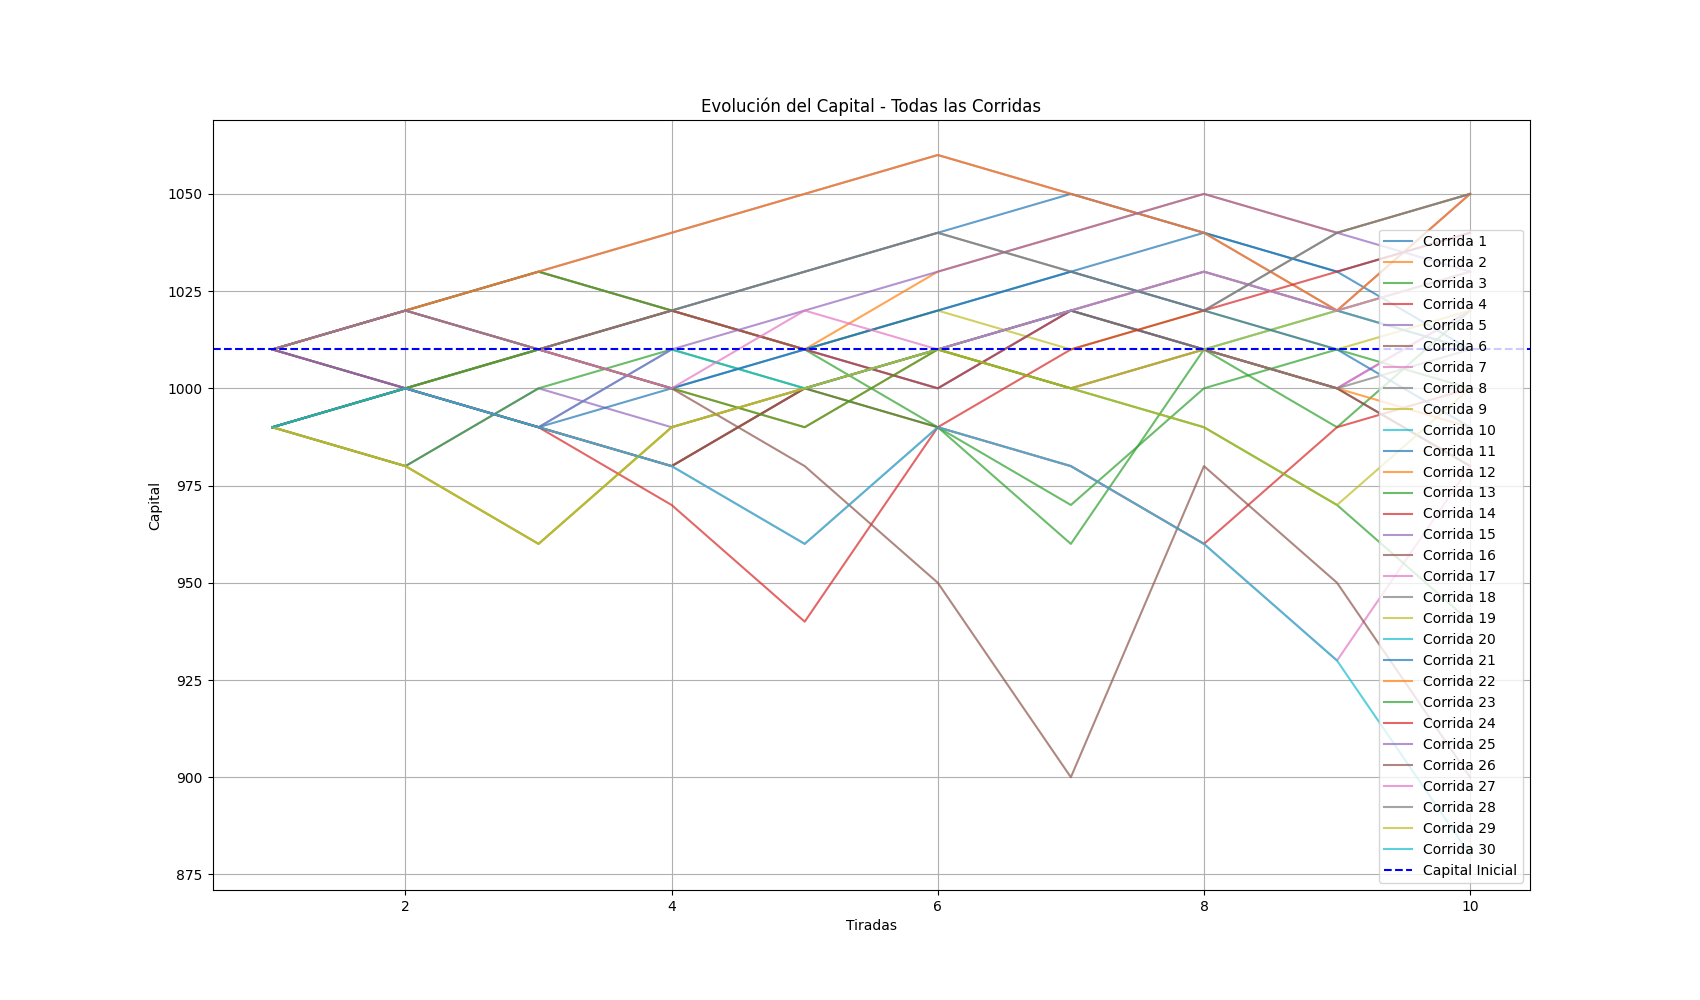
\includegraphics[width=0.85\textwidth]{./images/capital_todas_corridas_f_i.png}
    \caption{Fibonacci (infinito) - Capital en 30 corridas}
\end{figure}


% ====================
% Paroli
% ====================
\subsubsection*{Estrategia Paroli}


\begin{figure}[H]
    \centering
    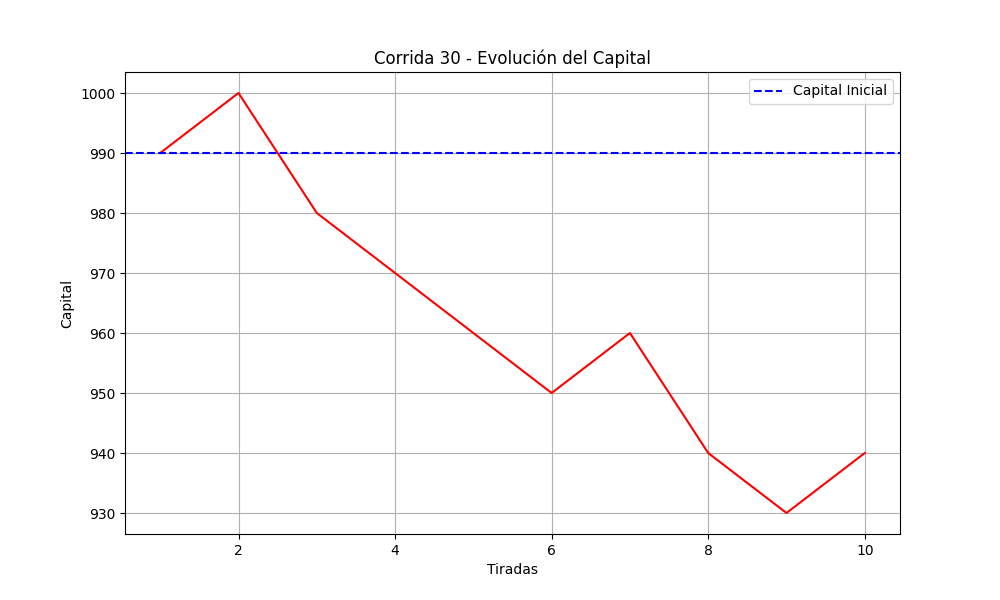
\includegraphics[width=0.8\textwidth]{./images/capital_corrida_30_p_f.png}
    \caption{Paroli (finito) - Evolución del capital en una corrida}
\end{figure}

\begin{figure}[H]
    \centering
    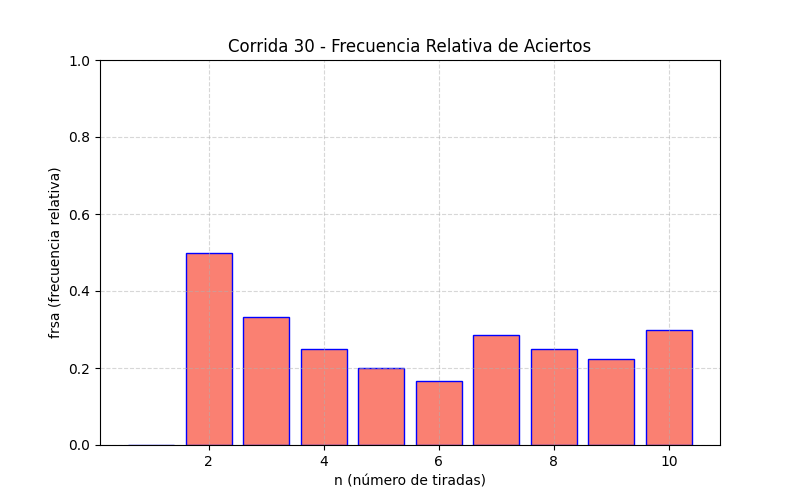
\includegraphics[width=0.7\textwidth]{./images/frsa_corrida_30_p_f.png}
    \caption{Paroli (finito) - Frecuencia relativa de aciertos}
\end{figure}

\begin{figure}[H]
    \centering
    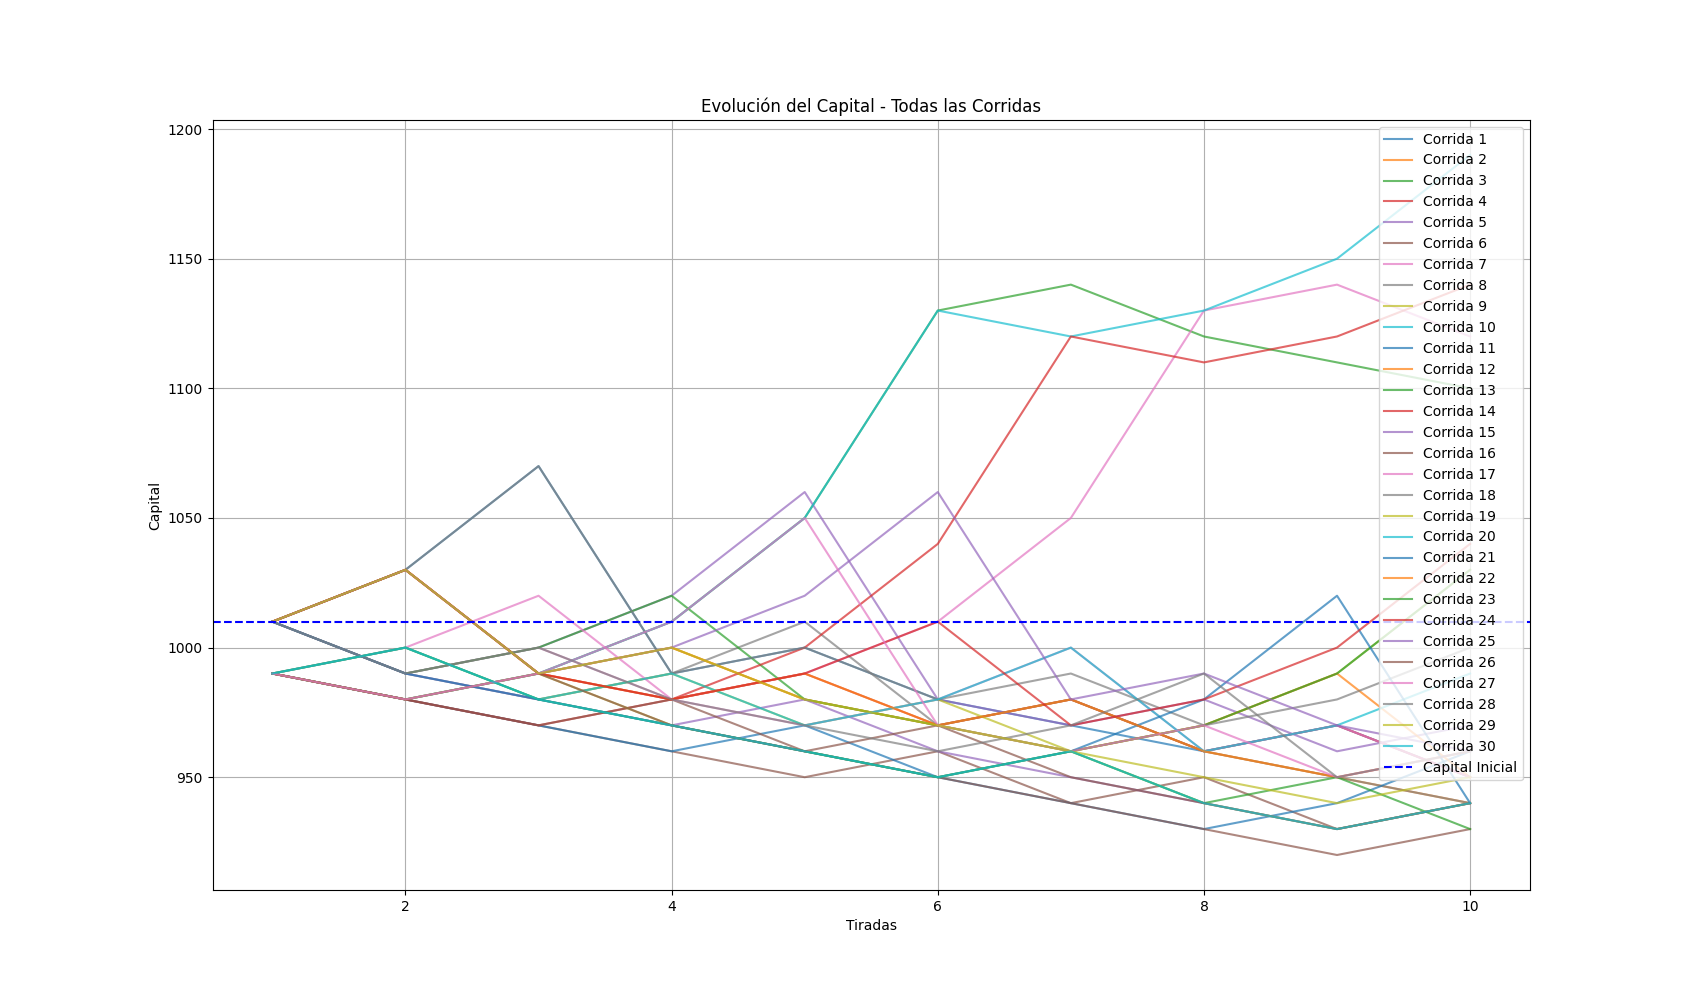
\includegraphics[width=0.85\textwidth]{./images/capital_todas_corridas_p_f.png}
    \caption{Paroli (finito) - Capital en 30 corridas}
\end{figure}

\begin{figure}[H]
    \centering
    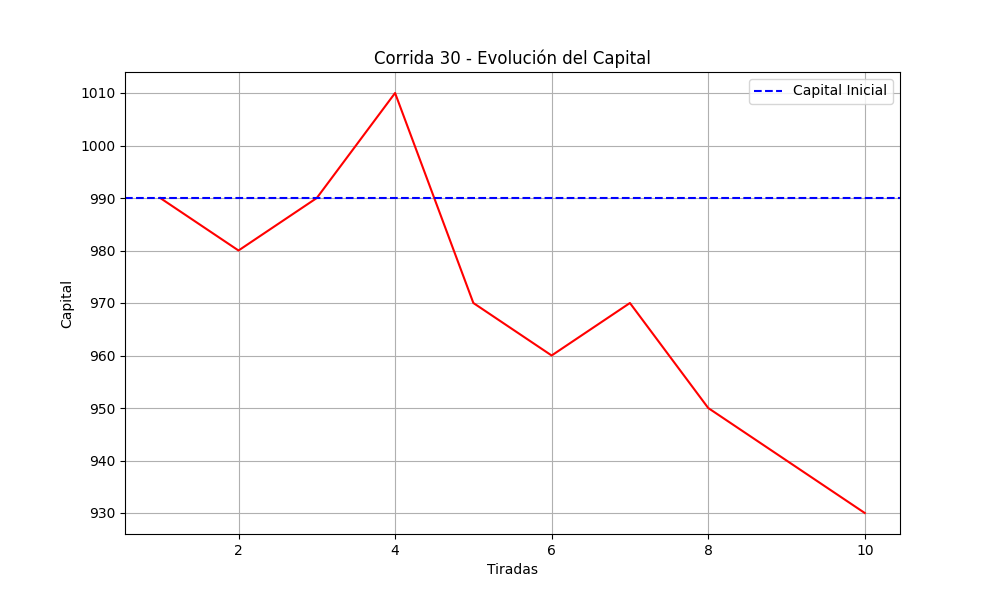
\includegraphics[width=0.8\textwidth]{./images/capital_corrida_30_p_i.png}
    \caption{Paroli (infinito) - Evolución del capital en una corrida}
\end{figure}

\begin{figure}[H]
    \centering
    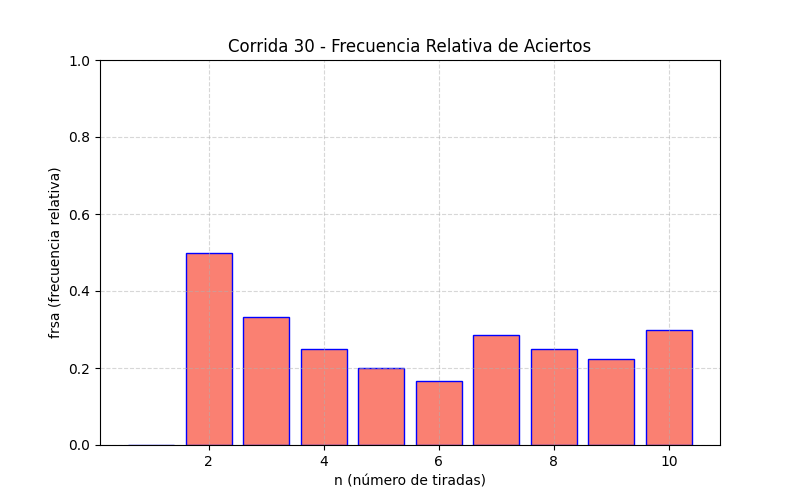
\includegraphics[width=0.7\textwidth]{./images/frsa_corrida_30_p_f.png}
    \caption{Paroli (infinito) - Frecuencia relativa de aciertos}
\end{figure}

\begin{figure}[H]
    \centering
    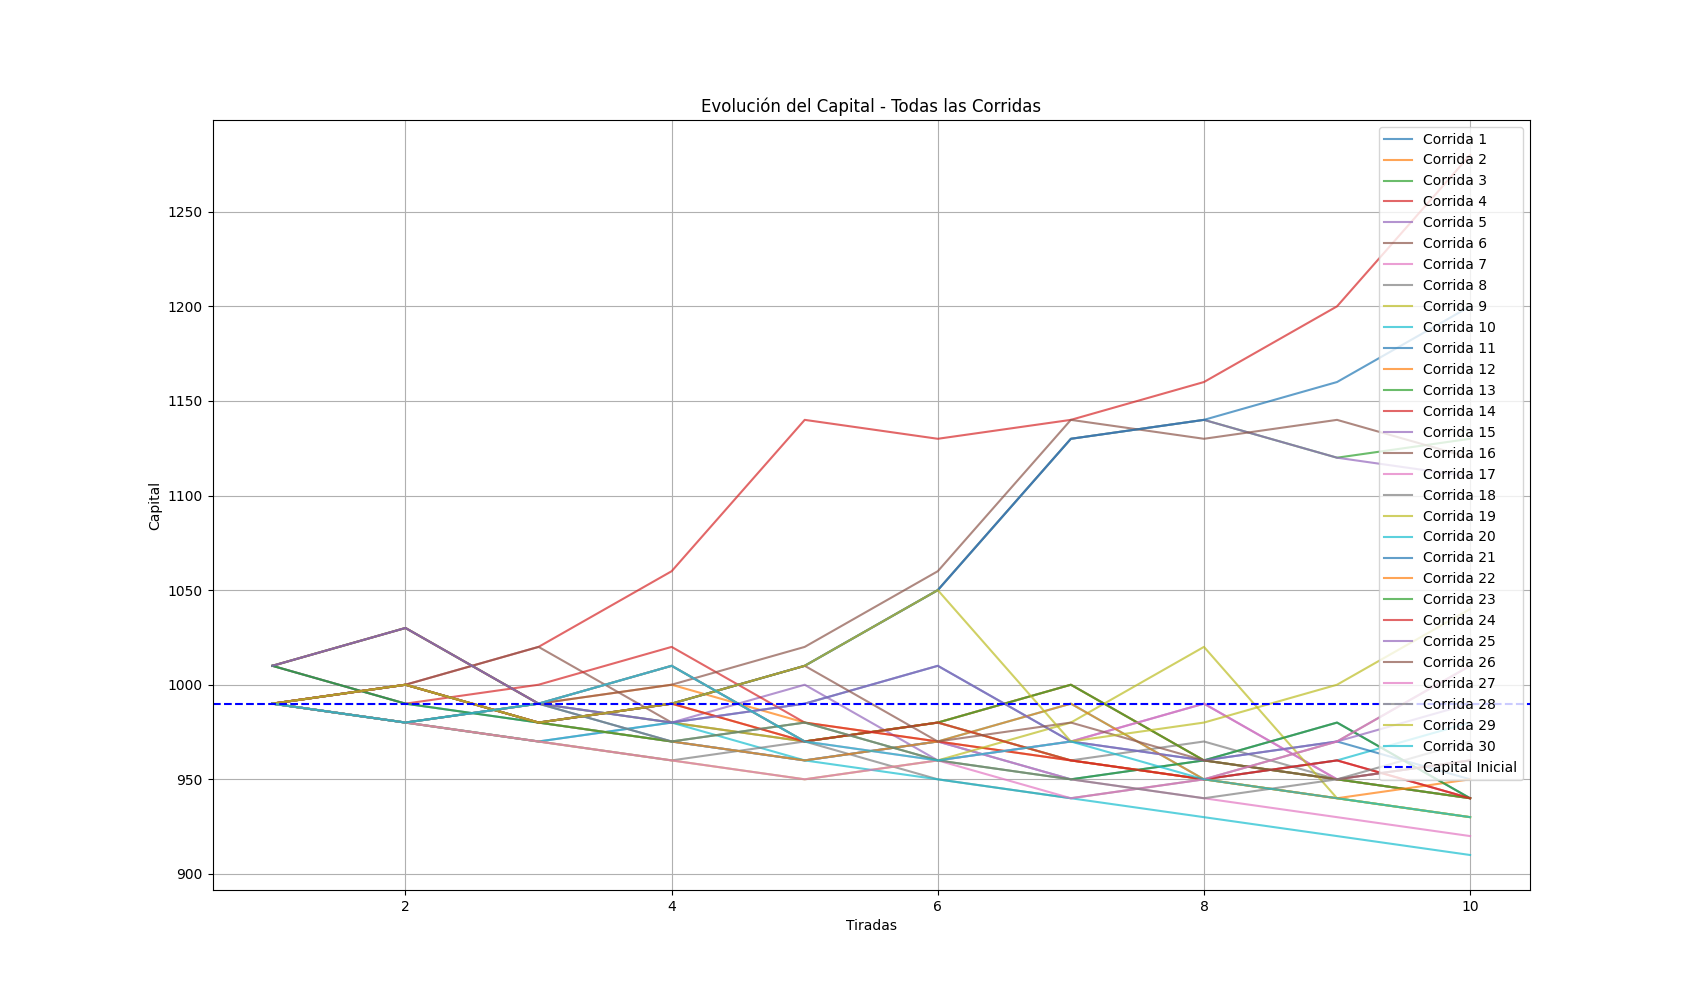
\includegraphics[width=0.85\textwidth]{./images/capital_todas_corridas_p_i.png}
    \caption{Paroli (infinito) - Capital en 30 corridas}
\end{figure}



\section{Conclusion general}
Las estrategias muestran comportamientos distintos dependiendo del capital disponible. 
\begin{itemize}

\item \textbf{Martingala: }
El objetivo es recuperar todas las pérdidas anteriores con una única victoria.

El riesgo con capital limitado es muy alto, ya que las apuestas se doblan después de cada pérdida, lo que puede agotar rápidamente los fondos disponibles. Esta estrategia es especialmente peligrosa porque una serie de pérdidas consecutivas puede llevar a la bancarota.

Capital infinito: Con capital infinito, la estrategia es teóricamente viable, pero teniendo en cuenta los límites que los casinos colocan a las apuestas, podría no serlo

\item \textbf{D'Alembert:} La estrategia D'Alembert tiene como objetivo es equilibrar las pérdidas y ganancias de una manera más controlada.

Esto hace que, con un capital finito puede ofrecer una gestión más segura en el largo plazo, ya que las apuestas no aumentan exponencialmente.

Con un capital infinito  la estrategia sigue siendo sostenible, ya que las apuestas no se incrementan rápidamente, lo que permite mantener un flujo de apuestas moderado y controlado.
\item \textbf{Fibonacci: }
Con capital limitado, esta estrategia puede llevar a una gran cantidad de pérdidas acumuladas antes de obtener una ganancia, lo que puede resultar riesgoso a largo plazo. Es más riesgosa que D'Alembert pero menos que Martingala.

Si el capital fuera infinito, la estrategia es viable teóricamente, ya que se basa en la idea de cubrir todas las pérdidas previas con una ganancia. Aún teniendo en cuenta esto,el crecimiento exponencial de las apuestas puede ser un desafío incluso con capital infinito.

\item \textbf{Paroli: }
A diferencia de la Martingala, la Paroli se enfoca en duplicar las apuestas tras cada victoria en lugar de cada pérdida. El objetivo es aprovechar las rachas ganadoras.

A pesar de ser una estrategia más conservadora que la Martingala, aún puede ser riesgosa si el jugador experimenta una racha de pérdidas, ya que necesitaría recuperar las ganancias perdidas con victorias consecutivas. Sin embargo, debido a que las apuestas solo aumentan tras una victoria, el riesgo no es tan elevado como con la Martingala.

Capital infinito: Si tuviera un capital infinito, la Paroli podría ser muy efectiva, ya que permite al jugador aprovechar las rachas ganadoras sin la amenaza de grandes pérdidas. El mayor reto sería si la secuencia de victorias no es lo suficientemente larga para obtener una ganancia significativa.
\end{itemize}

\subsection{Conclusiones generales}
\textbf{Capital finito:} Las estrategias más conservadoras como Dalembert y Paroli son mejores para un apostador con capital limitado, ya que no aumentan el riesgo de forma exponencial y permiten una gestión de dinero más controlada. La Martingala y Fibonacci pueden ser muy peligrosas con un capital finito, ya que pueden llevar a una rápida quiebra en caso de una serie de pérdidas consecutivas.

\textbf{Capital infinito:} Con un capital infinito, las estrategias como la Martingala y Fibonacci se vuelven viables teóricamente, ya que el jugador tiene el dinero necesario para cubrir las apuestas crecientes. Sin embargo, el comportamiento del jugador en términos de paciencia y el límite de las apuestas del casino siguen siendo factores importantes a considerar.

\end{document}